\documentclass[10pt]{article}
\usepackage[polish]{babel}
\usepackage[utf8]{inputenc}
\usepackage[T1]{fontenc}
\usepackage{amsmath}
\usepackage{amsfonts}
\usepackage{amssymb}
\usepackage[version=4]{mhchem}
\usepackage{stmaryrd}
\usepackage{graphicx}
\usepackage[export]{adjustbox}
\graphicspath{ {./images/} }
\usepackage{hyperref}
\hypersetup{colorlinks=true, linkcolor=blue, filecolor=magenta, urlcolor=cyan,}
\urlstyle{same}

\title{Zestaw 29 }

\author{}
\date{}


\begin{document}
\maketitle
\begin{enumerate}
  \item Wybieramy losowo cięciwę danego okręgu. Jakie jest prawdopodobieństwo, że będzie ona miała długość większą niż długość boku trójkąta równobocznego wpisanego w ten okrąg?
  \item Znajdź błąd w poniższym rozumowaniu:
\end{enumerate}

Udowodnimy, że nie istnieje żaden trapez. Załóżmy, że czworokąt ABCD jest trapezem o równoległych bokach AB i CD i oznaczmy długości tych boków odpowiednio przez \(a\) i \(b\). Następnie uzupełnijmy ten trapez do równoległoboku, jak na rysunku poniżej i poprowadźmy przekątną FE. Oznaczmy długość odcinka DG przez c, odcinka AH przez \(d\) a odcinka GH przez \(e\).\\
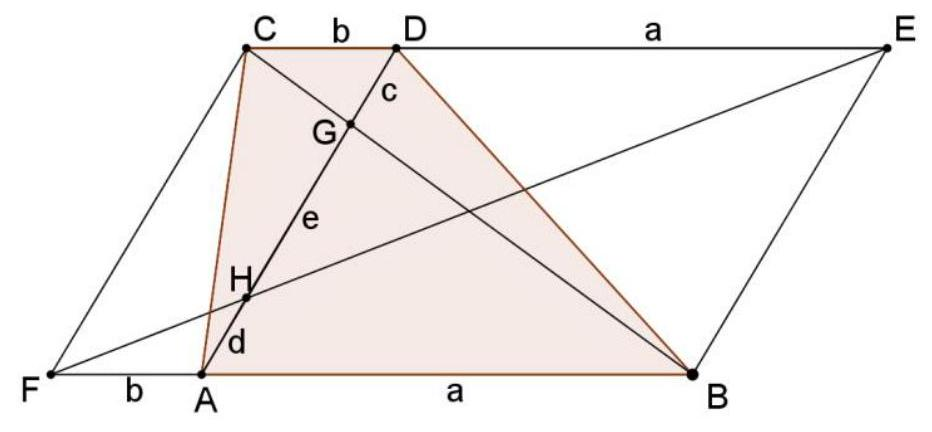
\includegraphics[max width=\textwidth, center]{2024_11_21_77e8d14deb5a0f880882g-1}

Z podobieństwa trójkątów CDG i ABG dostajemy: \(\frac{b}{c}=\frac{a}{d+e^{\prime}}\) a z podobieństwa trójkątów HED i FAH dostajemy: \(\frac{b}{d}=\frac{a}{c+e}\). Wyliczamy z obu tych równań \(e\), porównujemy do siebie i dostajemy:

\[
\begin{aligned}
& \frac{a c}{b}-d=\frac{a d}{b}-c . \\
& a c-b d=a d-b c \\
& a c-a d=-b c+b d \\
& a(c-d)=-b(c-d) \\
& a=-b
\end{aligned}
\]

Ponieważ obie liczby \(a\) i \(b\) są nieujemne, więc są równe zero, więc nie ma czworokąta o równoległych bokach!\\
3. Przy okrągłym stole siedzi kilku panów tak, że każdy ma dwóch sąsiadów. Każdy ma przy sobie pewną ilość złotówek. Pan A ma o złotówkę więcej niż Pan B, Pan B o złotówkę więcej niż Pan C i tak dalej. Pan A daje Panu B złotówkę. Następnie Pan B daje Panu C 2 złote i tak dalej. Każdy daje o złotówkę więcej niż dostał tak długo, jak długo jest to możliwe. Na końcu okazuje się, że jeden z panów ma cztery razy więcej pieniędzy niż pewien inny. llu panów siedzi przy stole?

Rozwiazania należy oddać do piatku 17 maja do godziny 13.00 koordynatorowi konkursu panu Jarosławowi Szczepaniakowi lub przestać na adres \href{mailto:jareksz@interia.pl}{jareksz@interia.pl} do soboty 18 maja do pótnocy.


\end{document}